\documentclass[journal]{IEEEtran}

\usepackage{blindtext}
\usepackage{cite}
\usepackage{graphicx}
\usepackage{array}
\usepackage{color}
\usepackage{tabularx}
\usepackage{epsfig}
\usepackage{amsmath}
\usepackage{amssymb}
\usepackage{bm}
\usepackage{wasysym}
\usepackage{circuitikz}
\usepackage{float}
\usetikzlibrary{arrows,shapes,calc,positioning}

\newcommand{\myscope}[2]
{\draw[thick,rotate=#2] (#1) circle (12pt)
(#1) ++(-0.35,-0.1) --++ (0.3,0.3) --++ (0,-0.3) --++(0.3,0.3) --++(0,-0.3);}

\begin{document}

\title{CSCE 221 \\ Problem Set 10}

\author{Jacob~Purcell,~\IEEEmember{Texas~A\&M,~Student}}

\maketitle
\section{}
	The following diagrams show the steps taken to balance the binary tree, all arrows indicate pointers, 
	blue shows formed connections, red shows broken connections, and orange shows cursor pointers that 
	are used for keeping track of nodes while the rotations occur. Eq. 1 will be used to calculate the 
	balance of the binary search tree. The null pointer has a height of -1. 
	\begin{equation}
		Balance = h_L - h_R
	\end{equation}
	and the condition must hold that
	\begin{equation}
		\mid Balance \mid \le 1
	\end{equation}

	Figure 1 unbalance starts at the left child of the root node, which has a balance of $3$ since the left 
	child has a height of 2 and the right child is the null pointer, so a right rotation is performed. 

\begin{figure}[h!]
	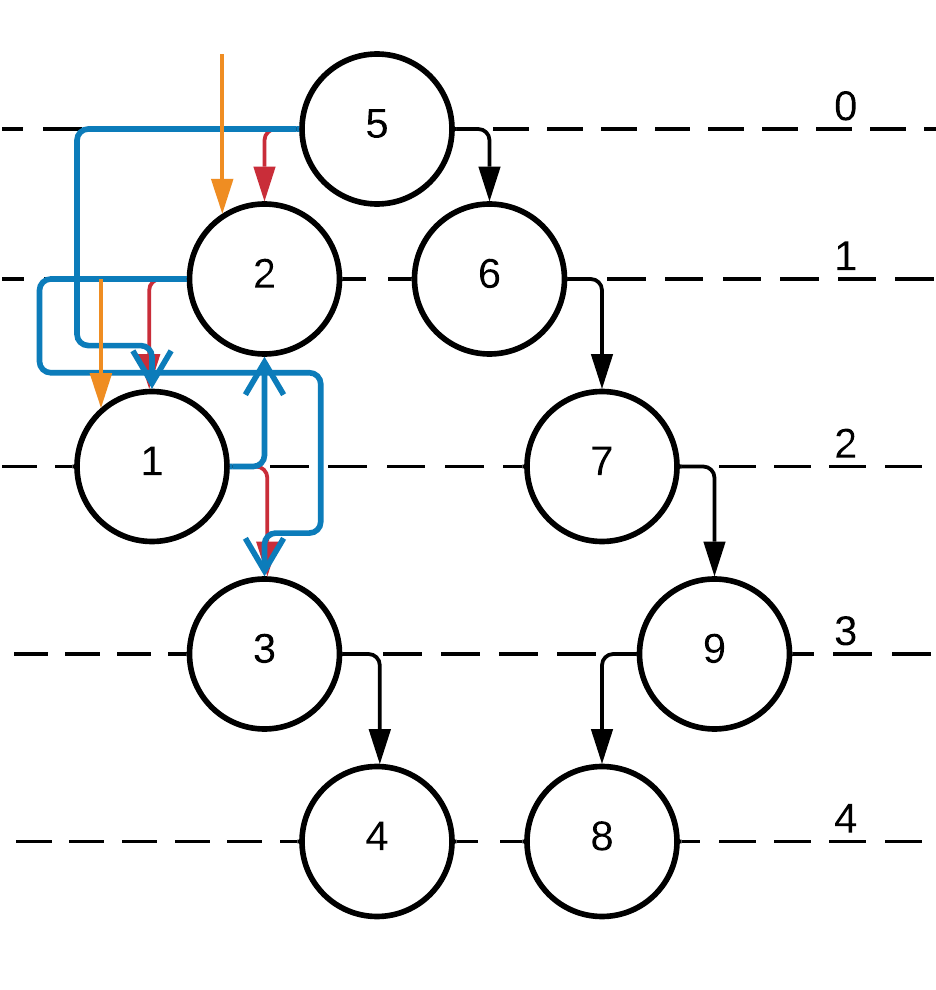
\includegraphics[scale = 0.2]{avl11.png}
	\caption{The initial tree plus its first rotation.}
\end{figure}

Now the right child of the first unbalanced node($Left~subtree,~Depth = 1$) has a height of 2 with the left 
child being the null pointer(balance $-3$) so a left rotation is performed.

\begin{figure}[h!]
	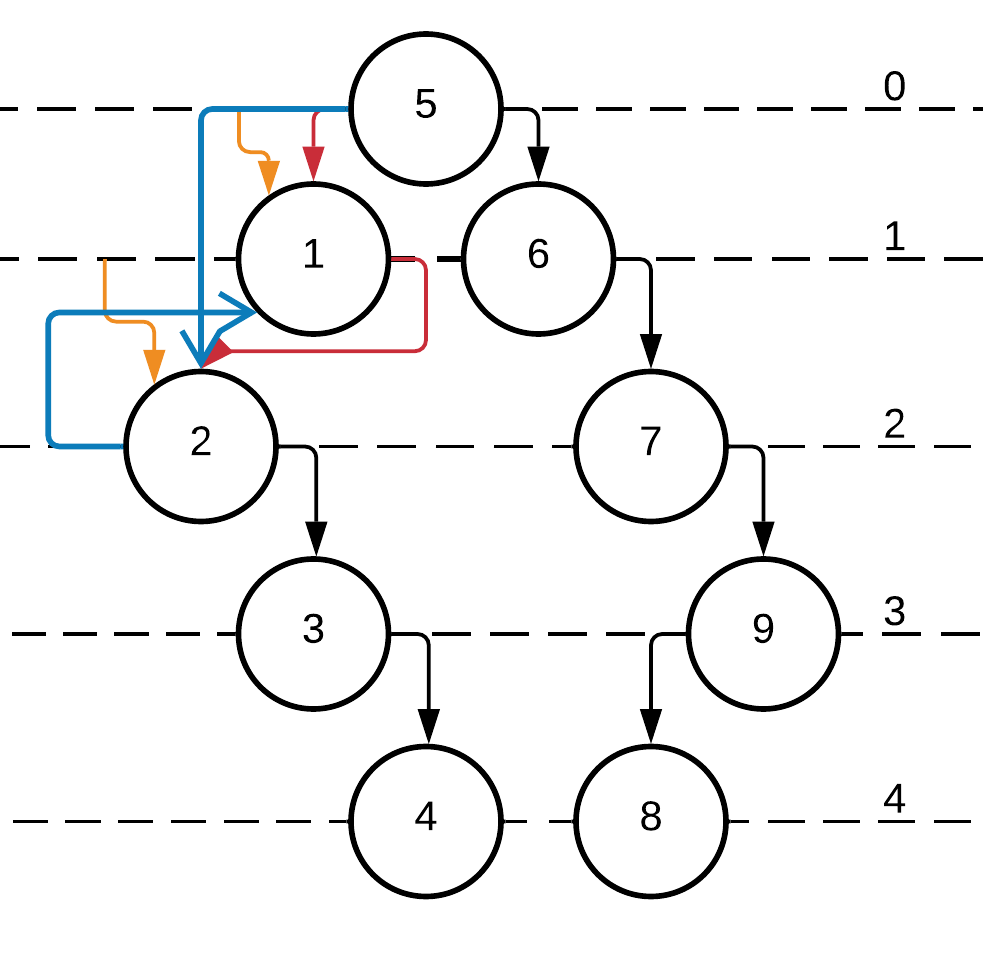
\includegraphics[scale = 0.2]{avl12.png}
	\caption{Result of the preceeding rotation and a left rotation at the same position.}
\end{figure}

This completes the first rebalancing operation, Left-Right Rotation. Scanning the rest 
of the root's left subtree, the following values correspond to the the balances

$$2:~-1$$
$$1:~0$$
$$3:~-1$$
$$4:~0$$

so the root's left subtree is balanced. The next imbalance occurs at the first node 
on the root's right subtree, with a balance of $-3$, so a left rotation must be performed.


\begin{figure}[h!]
	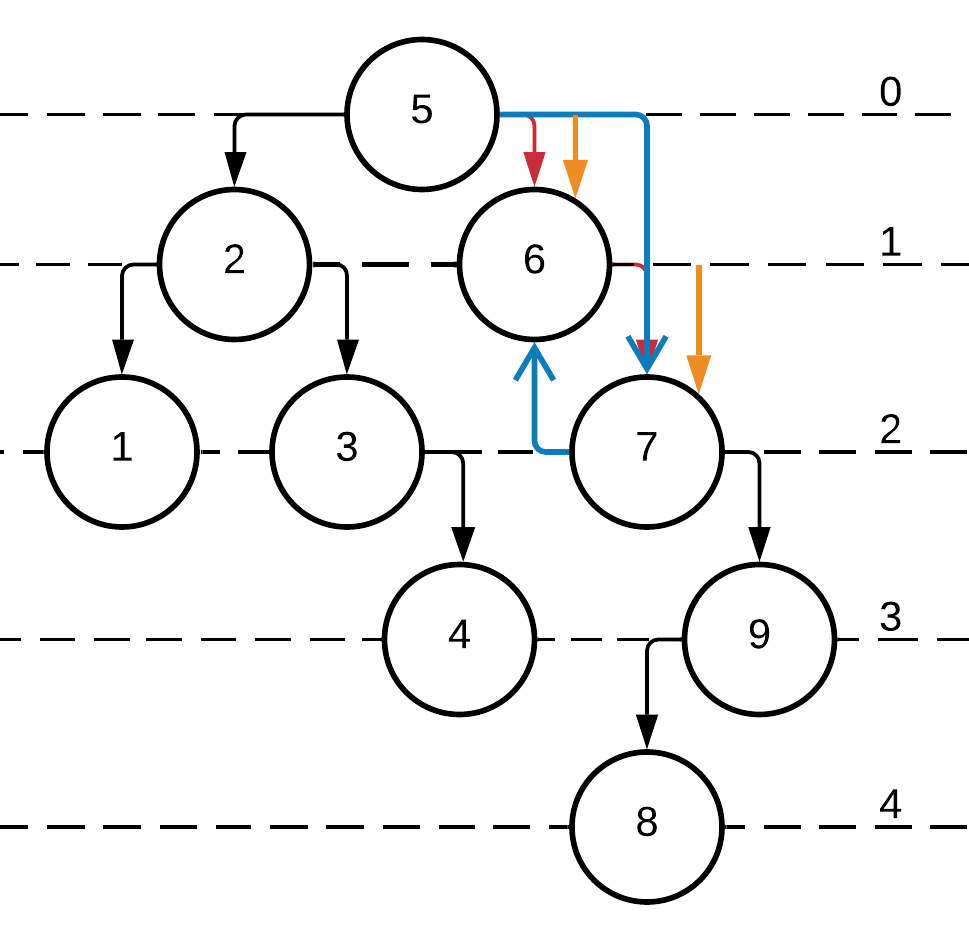
\includegraphics[scale = 0.2]{avl13.png}
	\caption{Results of preceeding rotation and shows the next left rotation.}
\end{figure}

This completes the left rotation 
operation. The balance of the root's left subtree is now 

$$7:~-1$$
$$6:~0$$
$$9:~1$$
$$8:~0$$

with the root having a balance of $0$. The tree is now fully balanced, however this process only required 2($RL,~LL$)
of the 4 operations($RL,~LR,~RR,~LL$).

\begin{figure}[h!]
	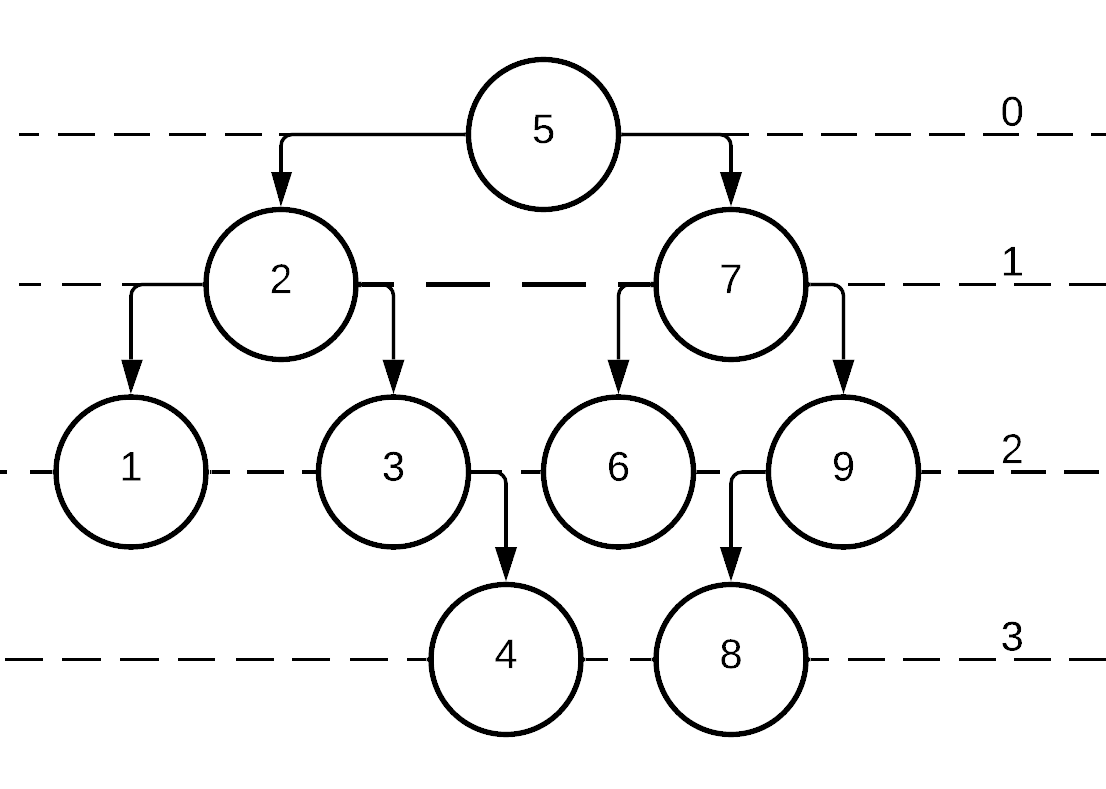
\includegraphics[scale = 0.2]{avl14.png}
	\caption{AVL tree.}
\end{figure}

\section{}

As shown in Fig. 5, the tree is initially balanced but once 12 is deleted, 
the node that carries 11 has a balance of $2$, so a right rotation must 
be performed(Fig. 6). Now the root node has a balance of $2$ so a 
right rotation must be performed at the root node(Fig. 7). The tree is now balanced 
and 12 has been removed(Fig. 8).


\begin{figure}[h!]
	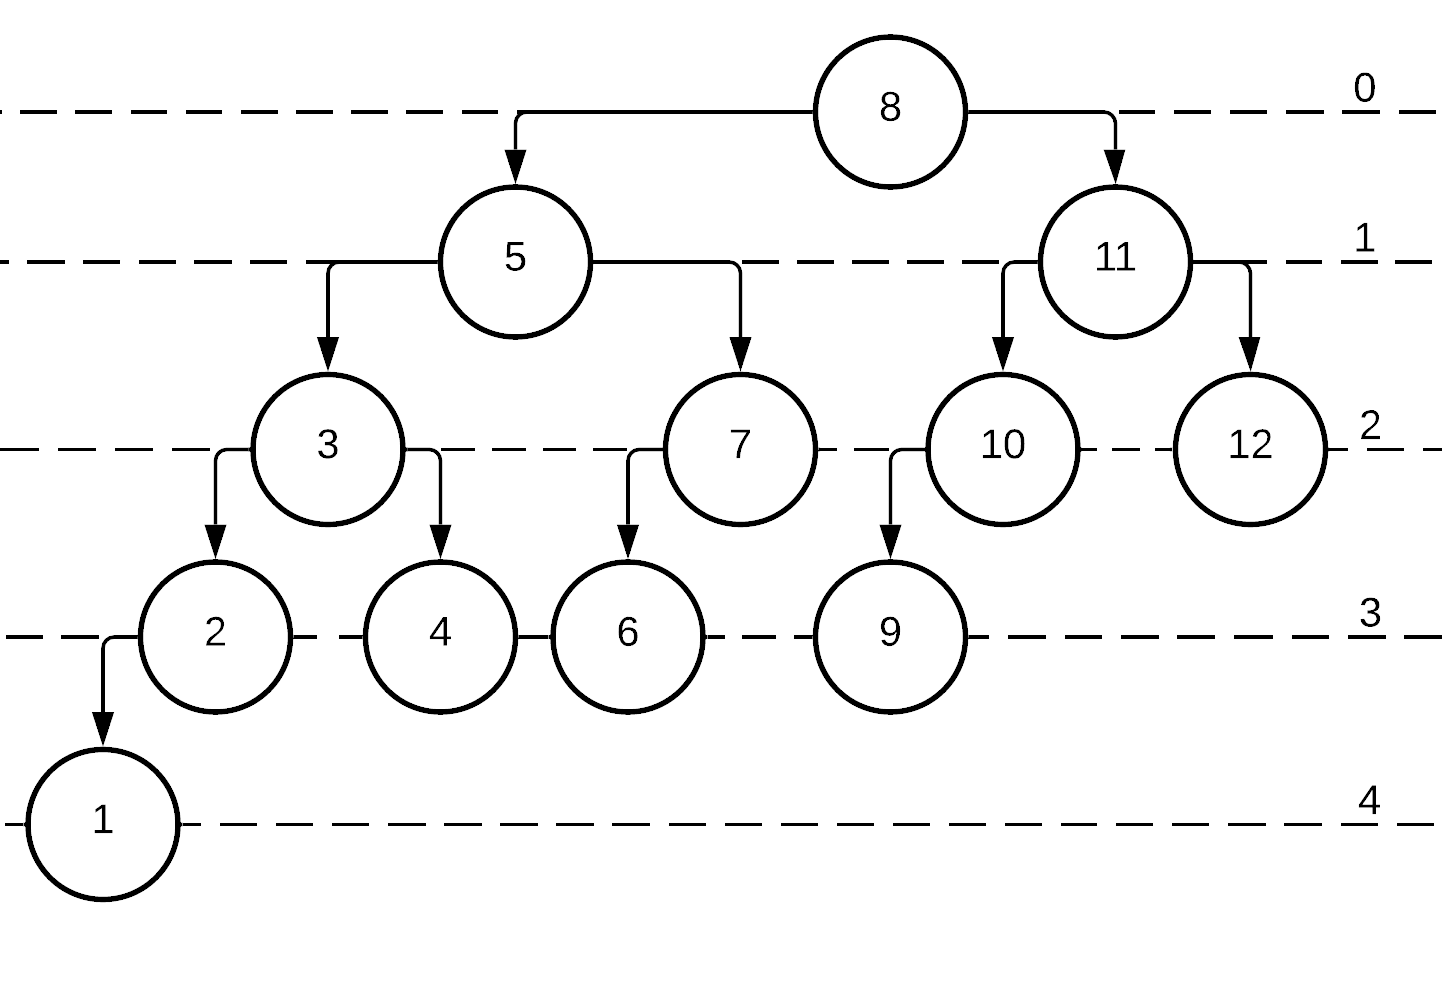
\includegraphics[scale = 0.16]{avl21.png}
	\caption{Initial AVL tree.}
\end{figure}


\begin{figure}[h!]
	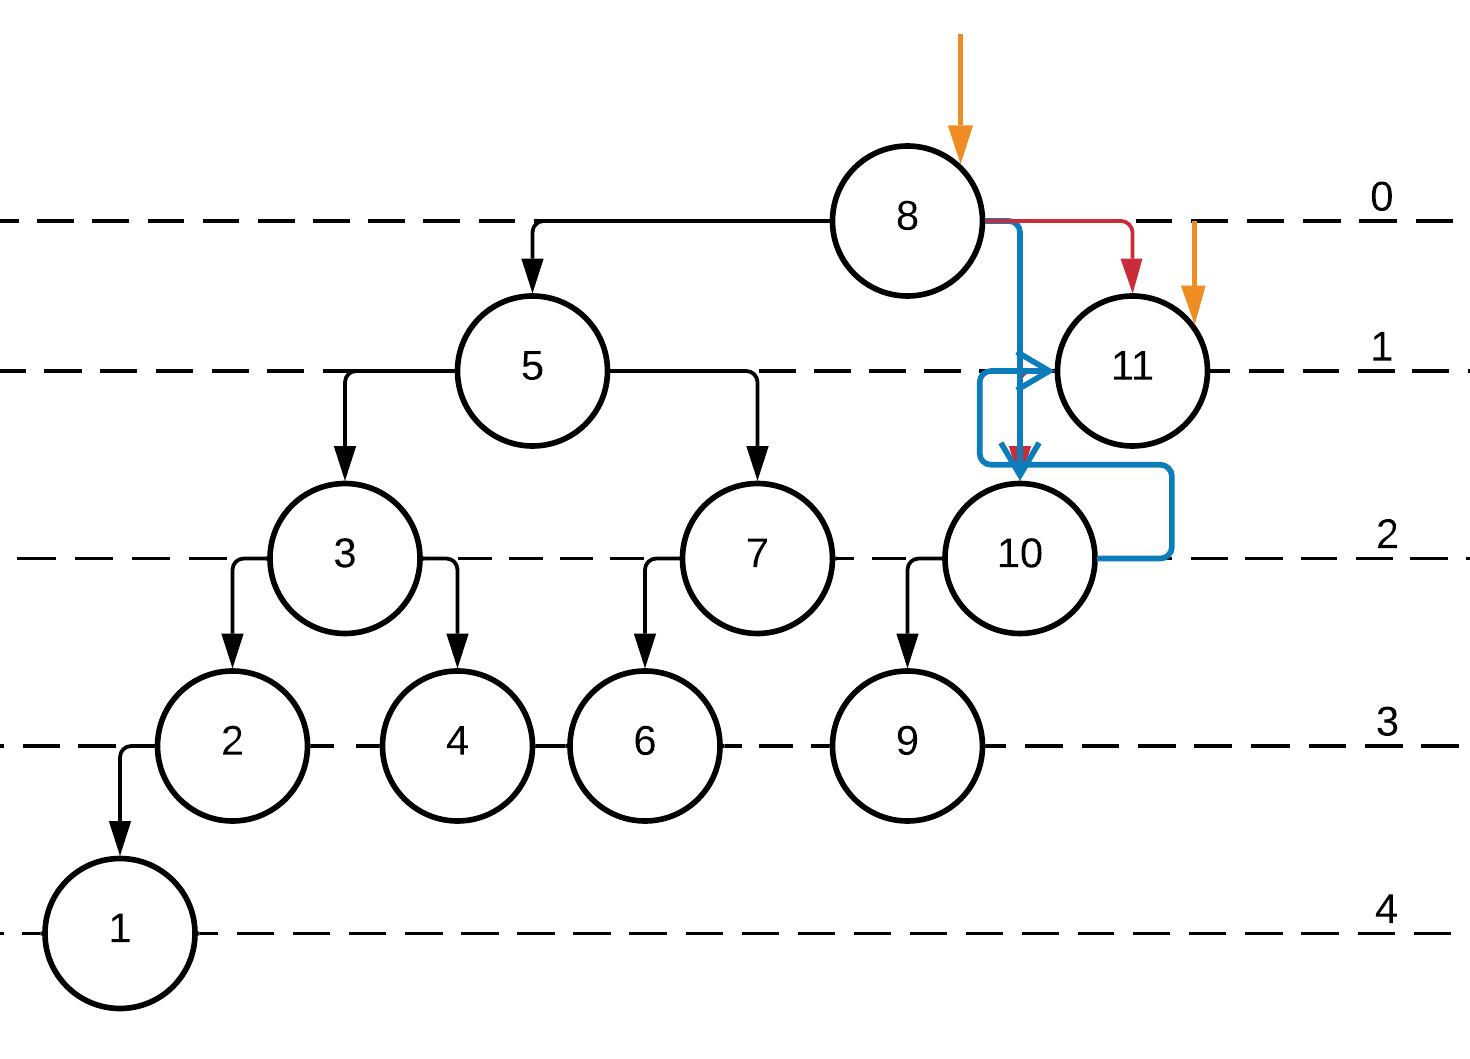
\includegraphics[scale = 0.15]{avl22.png}
	\caption{Deleted value unbalanced the left subtree, therefore a right rotation is performed.}
\end{figure}


\begin{figure}[h!]
	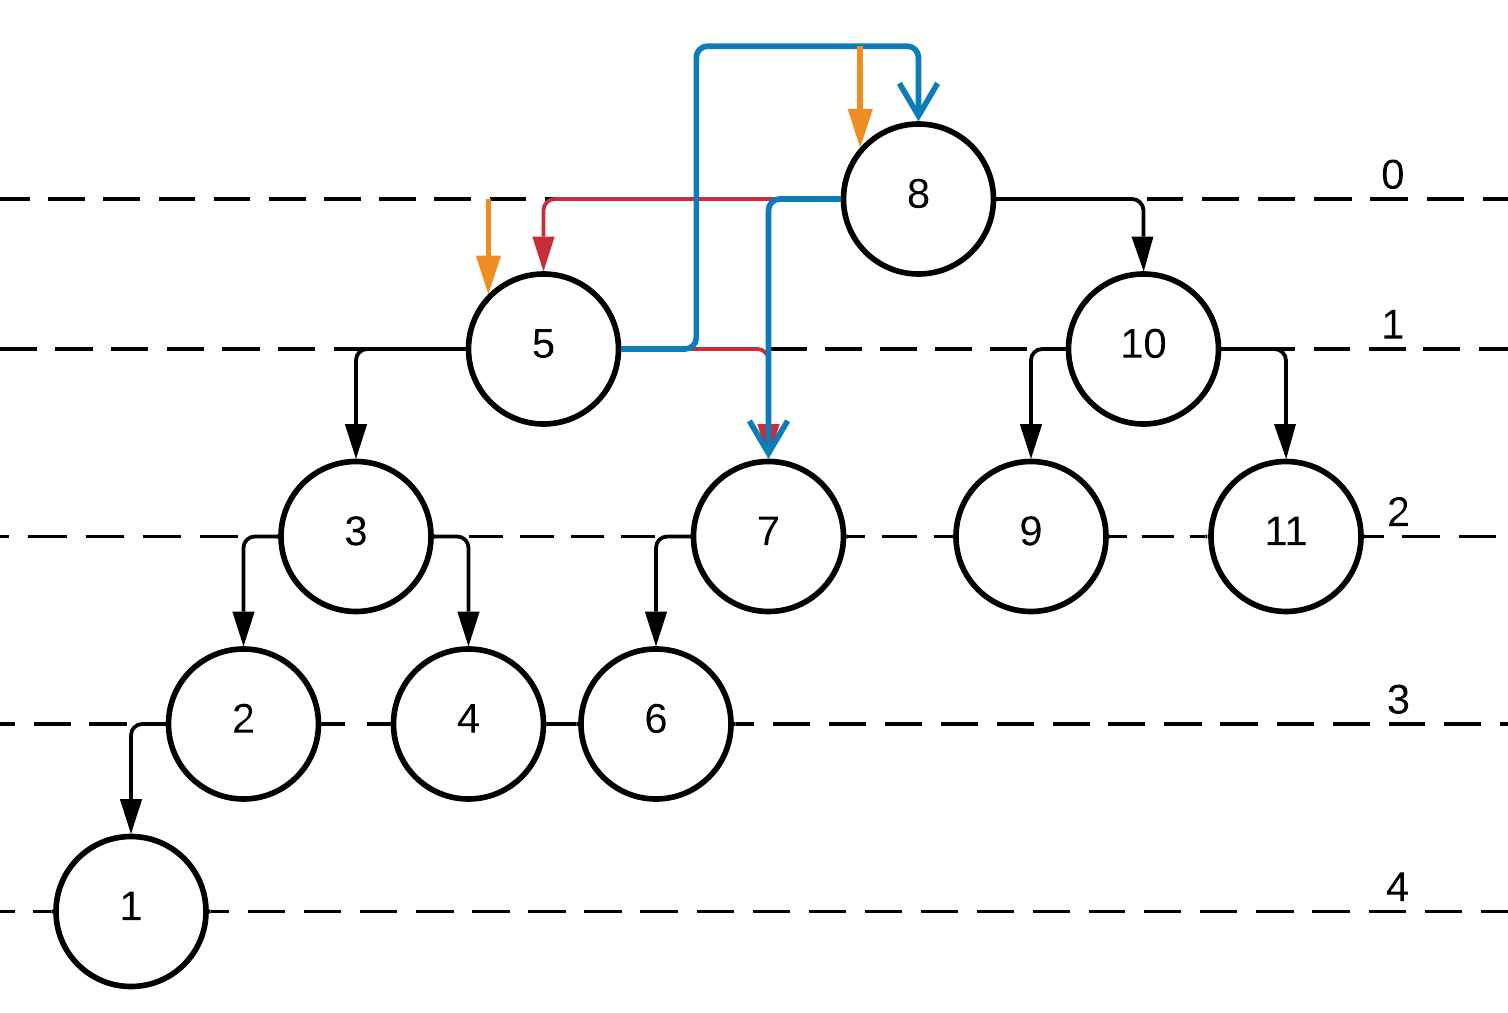
\includegraphics[scale = 0.15]{avl23.png}
	\caption{Another rotation must be performed to maintain tree integrity.}
\end{figure}


\begin{figure}[h!]
	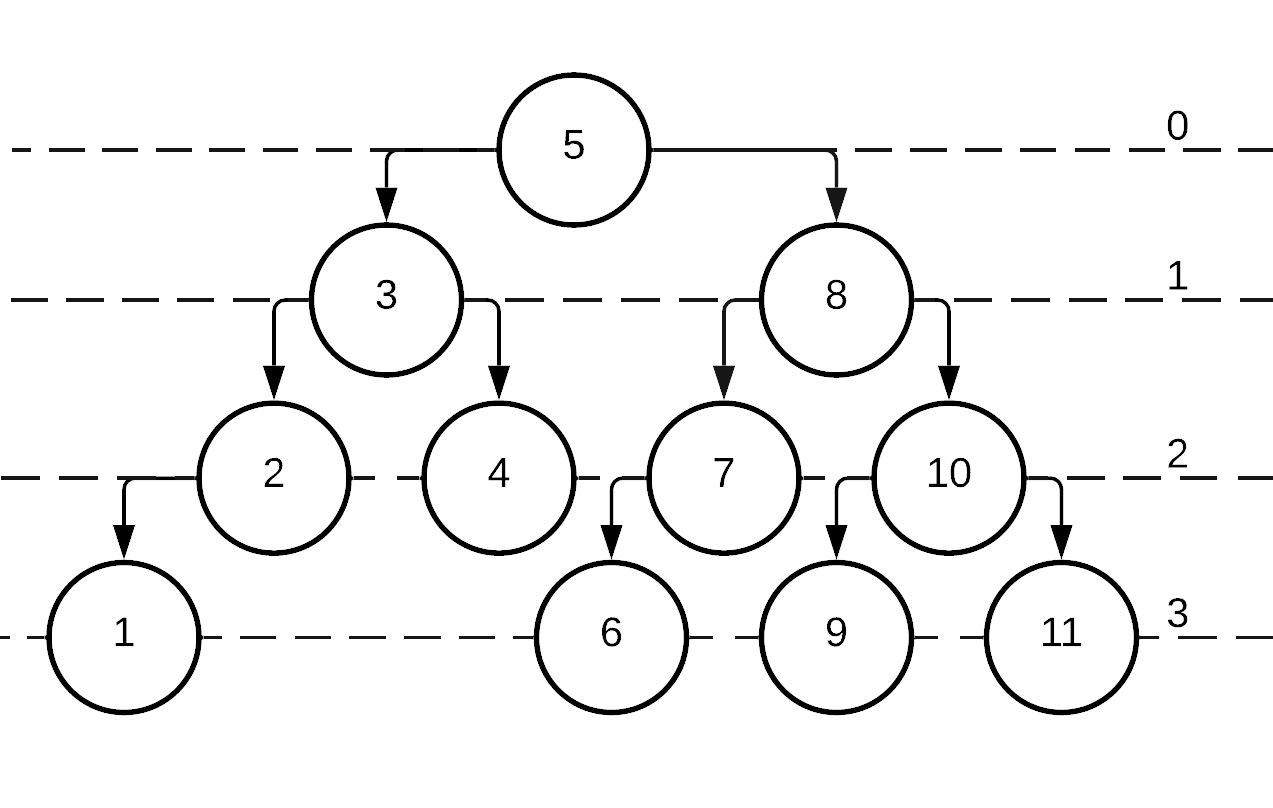
\includegraphics[scale = 0.18]{avl24.png}
	\caption{Final result of removing 12.}
\end{figure}

\section{}

As proven in Problem Set 9, the equation relating number of nodes in a tree is

\begin{equation}
	Nodes = 2^{height - 1}-1
\end{equation}

To find the minimum number of nodes in a tree with height 13, first we find the full tree at height 12, then add one leaf node.
This results in the following equation,

$$Nodes = 2^{12 - 1} - 1 + 1$$
$$Nodes = 2^{11}$$
$$Nodes = \boxed{2048}$$

\section{}

An example of a double rotation is included in "mainps10.cpp," the definition of this rotation is in "tree\_functions.h."

\end{document}
